\section{LHC: Gran Colisionador de Hadrones}

El LHC (\textit{Large Hadron Collider}) es el acelerador de partículas más grande del mundo que se encuentra en la frontera franco-suiza. Se encuentra en las instalaciones del CERN, la Organización Europea para las Investigaciones Nucleares y se trata de un anillo de 27 diámetros de circunferencia enterrado a 100 metros bajo el suelo. Se contruyó entre 1998 y 2008 y ha sufrido a lo largo de casi 20 años sucesivas mejoras, entre ellas la que está sucediendo en estos momentos: el High Luminosity - LHC que aumentará la energía de las colisiones a 14 TeV frente a los 3,5 TeV de energía que tenían las primeras colisiones que ocurrieron en el LHC en el 2010. A lo largo del LHC hay 4 puntos de cruce donde las partículas chocan. Alrededor de estos puntos se colocan los detectores de partículas, entre los cuales destacan ALICE, ATLAS, LHC-b y CMS. En el LHC se estudian generalmente colisiones protón-protón, pero también se estudian colisiones entre iones pesados para observar estados exóticos de la materia como el Plasma de Quarks y Gluones.\\


En el interior del anillo del acelerador se crea un ultra-vacío para evitar que las partículas aceleradas choquen con moléculas del aire. Los protones se ven acelerados y desviados gracias a miles de imanes que se reparten por todo el acelerador. Por ejemplo, se utilizan 1232 imanes dipolares de 15 metros de longitud que desvían los haces y 392 imanes cuadrupolares de entre 5 y 7 metros que enfocan los hacen. Debido al diminuto tamaño de las partículas aceleradas, se utiliza otro tipo de imán para condensar las partículas y la probabilidad de que las partículas del haz choquen sea mayor.\\

Al LHC se le introducen haces de protones (o de iones pesados) que viajan en direcciones contrarias, son acelerados a velocidades de 99,9999991$\%$ de la velocidad de la luz y colisionan en unos puntos específicos. Al colisionar, toda la energía acumulada de las partículas se emplea en crear nuevas partículas que son detectadas por los diferentes experimentos. Cabe destacar que muchas de las partículas que se crean tienen un tiempo de vida extremadamente corto, por lo que la única manera de observarlas es mediante este tipo de aceleradores.\\
IMÁGEN?
\url{https://www.i-cpan.es/es/content/el-gran-colisionador-de-hadrones-lhc-del-cern}

\section{Experimento CMS}

En uno de los puntos de cruce del LHC se encuentra el CMS (\textit{Compact Muon Solenoid}), un detector de uso general cuyo objetivo es observar gran cantidad de partículas y fenómenos distintos. El detector CMS se dispone de manera cilíndrica con tamaño de 21 metros de largo y 16 metros de ancho. El CMS se caracteriza además por la buena caracterización de muones y de reconstruir de manera muy eficiente el momento, además de por un solenoide de 4 T que se encuentra entre dos capas.\\

La disposición del detector se divide en 4 capas de detectores. La capa más interna se denomina \textit{tracker} y consiste de 25000 detectores de silicio de micro-bandas que se colocan de manera que se obtiene la granularidad y precisión que requieren el experimento. En esta capa se mide el impacto de partículas cargadas y la posición de vértices secundarios.\\

Alrededor del \textit{tracker} se encuentra el Calorímetro Electromagnético (ECAL). El objetivo principal del ECAL es la medición de la energía de las partículas electromagnéticas que lo atraviesan. Está compuesto por cristales de PbWO$_4$, un material extremadamente denso para que las partículas depositen su energía. A continuación se sitúa el Calorímetro Hadrónico (HCAL) que, como su propio nombre indica, detecta hadrones y mide de manera indirecta el paso de neutrinos. Este HCAL está compuesto de materiales densos tal y como latón o acero. En ambos calorímetros se encuentra además centelladores y fotodiodos para la lectura.\\

Después de los calorímetros se coloca el gran solenoide. Como ya se ha mencionado, este imán genera un campo magnético de 4 T. Las partículas que surgen de las colisiones son extremadamente energéticas, así que es muy complicado desviarlas. Esa es la razón de que el solenoide del experimento CMS tenga un campo magnético tan grande, ya que esto permite determinar cuánto se desvían de su trayectoria inicial (medida de la razón carga/masa) y tener una buena medida del momento de partículas muy energéticas.\\

Una de las tareas en las que se especializa el experimento CMS es, como viene indicado en su nombre, la detección y reconstrucción de muones. El detector más externo del experimento, la cámara de muones, se centra en ellos. Los muones son capaces de atravesar varios metros de hierro sin depositar energía, por lo que es muy complicado detectarlos en los calorímetros o en el \textit{tracker}. Para identificarlos, se utilizan varios tipos de detectores: los tubos de deriva (DT), las cámaras de tiras de cátodos (CSC), las cámaras de placas resistivas (RPC) y multiplicadores de gas de electrones (GEM).

\begin{figure}[h!]
    \centering
    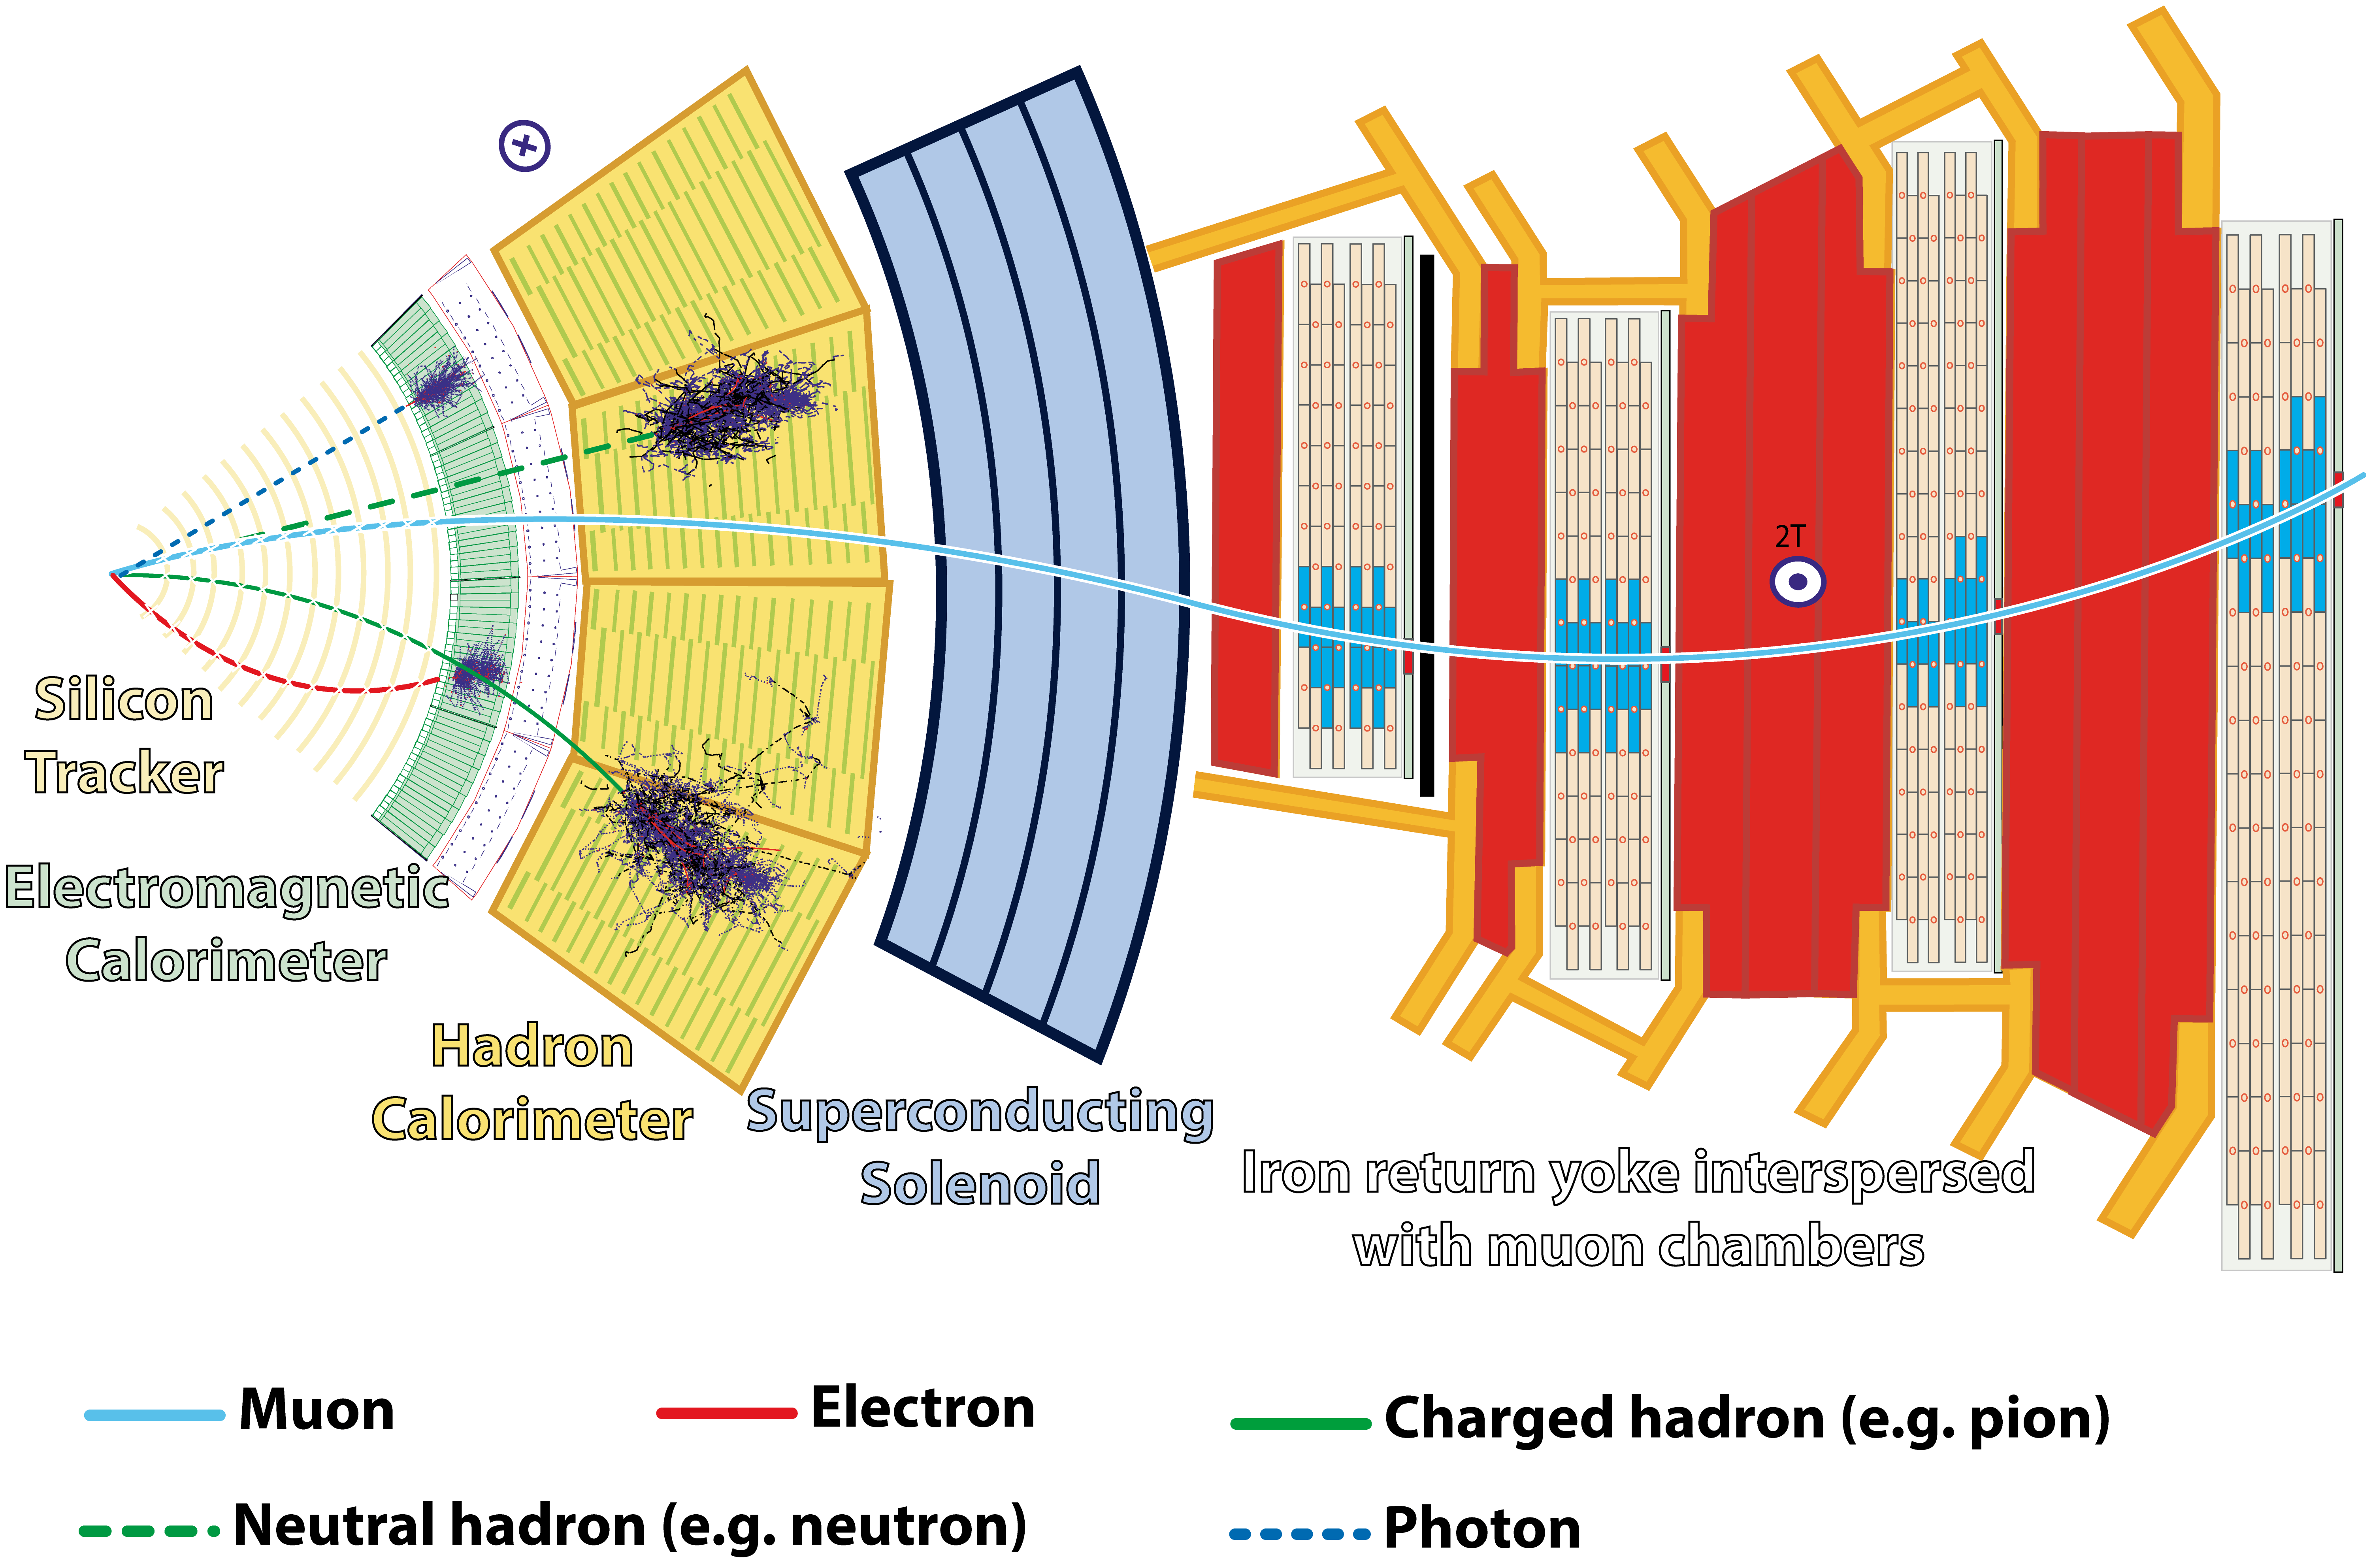
\includegraphics[width=0.5\linewidth]{CMSslice_whiteBackground (1).png}
    \caption{Caption}
    \label{fig:CMS_capas}
\end{figure}



\url{https://twiki.cern.ch/twiki/bin/view/CMSPublic/WorkBookCMSExperiment}
